\section{Zadanie 2}

\subsection{Implementacja główna}

\begin{lstlisting}[linewidth=16.0cm][caption={[Skrypt main, wykonujący kod główny]}]
classes_count = 5;
% Wczytywanie zdjec dla wybranej liczy klas
images_arrays = getAllImages(classes_count);
	
J = [4, 10, 20, 30];
iterations = 10;
	
% Wektor zawierajacy klasy kolejnych obrazow
images_classes = [];
for i = 1:classes_count
	images_classes =[images_classes; ones(10,1).*i];
end
	
% Petla glowna
for j_val = 1:4
	grouping_results = zeros([iterations 4]);
	classification_results = zeros([iterations 4]);
	
	for i = 1 : iterations
		% Redukcja wymiarow
		[V, pca_images_arrays, D] = myPCA(images_arrays', J(j_val));
		
		% Grupowanie za pomoca k-srednich
		g_result = getGroupingResults(
		images_arrays, pca_images_arrays, classes_count, 
		images_classes);
		grouping_results(i,:) = g_result;
		
		% Klasyfikacja z uzyciem k-NN
		c_result = getClassificationResults(
		images_arrays, pca_images_arrays, classes_count, 
		images_classes);
		classification_results(i,:) = c_result;
	end
	
	% Zapis wynikow do plikow
	(...)
end
\end{lstlisting}

\begin{lstlisting}[linewidth=16.0cm]
function [V, newX, D] = myPCA(X, J)
	X = bsxfun(@minus, X, mean(X,2));
	C = (X*X')./(size(X,2)-1);
	
	[V, D] = eigs(C,J);
	[D, order] = sort(diag(D), 'descend');
	V = V(:, order);
	newX = V'*X;
end
\end{lstlisting}


\subsection{Implementacja grupowania}

\begin{lstlisting}[linewidth=16.0cm]
function result = getGroupingResults(images_arrays, pca_images_arrays, 
	clusters, images_classes)
	
	% Uruchomienie grupowania k-srednich,
	% Zapis wynikow i czasu trwania
	tic;
	groups = kmeans(images_arrays, clusters);
	default_time = toc;
	tic;
	groups_pca = kmeans(pca_images_arrays', clusters);
	pca_time = toc;
	
	% Obliczenie skutecznosci grupowania i jej normalizacja
	default_acc = AccMeasure(images_classes, groups)/100.0;
	pca_acc = AccMeasure(images_classes, groups_pca)/100.0;
	
	result = [default_acc, pca_acc, default_time, pca_time];
end
\end{lstlisting}

\subsection{Implementacja klasyfikacji}

\begin{lstlisting}[linewidth=16.0cm]
function result = getClassificationResults(images_arrays, pca_images_arrays,
 classes_count, images_classes)

	% Uruchomienie klasyfikacji k-NN,
	% Zapis wynikow i czasu trwania
	tic;
	model = fitcknn(images_arrays, images_classes);
	cv_model = crossval(model,'KFold',classes_count);
	default_time = toc;
	tic;
	model_pca = fitcknn(pca_images_arrays', images_classes);
	cv_model_pca = crossval(model_pca,'KFold',classes_count);
	pca_time = toc;
	
	% Obliczenie skutecznosci grupowania
	cv_model_loss = kfoldLoss(cv_model);
	default_acc = 1 - cv_model_loss;
	cv_model_pca_loss = kfoldLoss(cv_model_pca);
	pca_acc = 1 - cv_model_pca_loss;
	
	result = [default_acc, pca_acc, default_time, pca_time];
\end{lstlisting}



\begin{lstlisting}[linewidth=16.0cm]

\end{lstlisting}

\subsection{Wyniki}

\subsubsection{Grupowanie}

\begin{figure}[H]
	\centering
	\hspace*{-0.8in}
	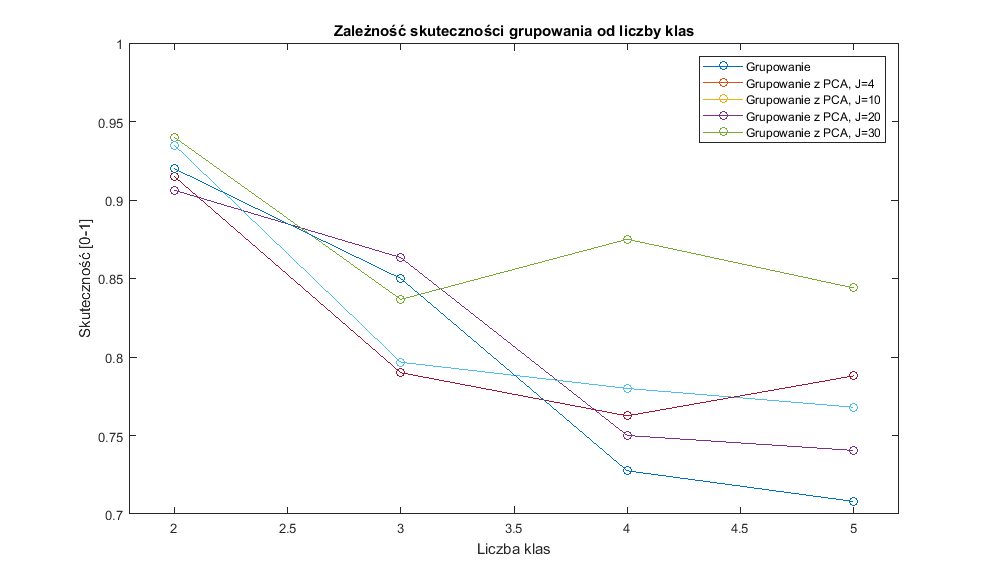
\includegraphics[scale = 0.7]{img/acc_from_classes_group.png}
	\caption{Skuteczność grupowania dla wymiarów pełnych i zredukowanych}  
	\label{rys:acc_from_classes_group} 
\end{figure}

\begin{figure}[H]
	\centering
	\hspace*{-0.8in}
	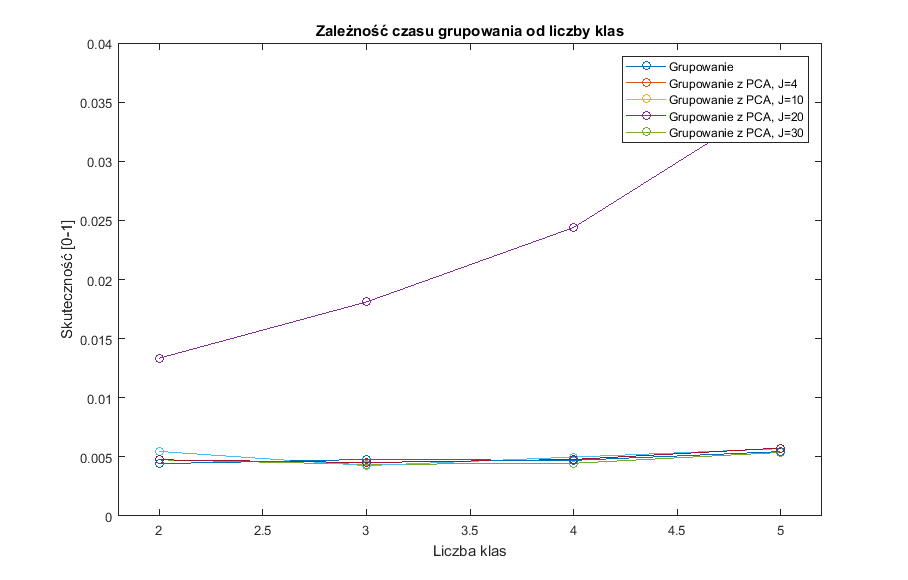
\includegraphics[scale = 0.7]{img/time_from_classes_group.png}
	\caption{Czas grupowania dla wymiarów pełnych i zredukowanych}  
	\label{rys:time_from_classes_group} 
\end{figure}

\subsubsection{Porównanie klasyfikacji i grupowania}

\begin{figure}[H]
	\centering
	\hspace*{-0.8in}
	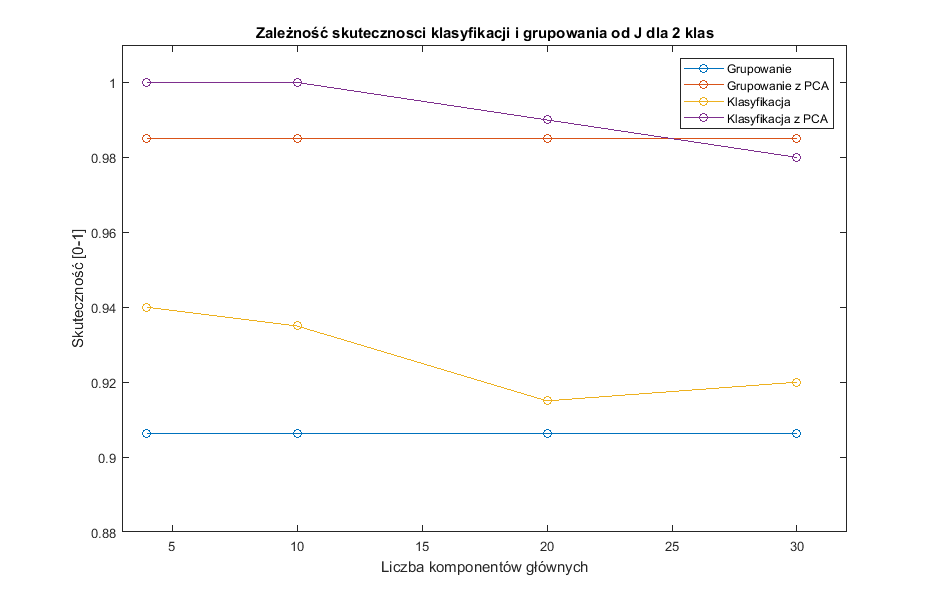
\includegraphics[scale = 0.7]{img/acc_from_J_2classes.png}
	\caption{Skuteczność grupowania i klasyfikacji dla 2 klas}  
	\label{rys:acc_from_J_2classes} 
\end{figure}

\begin{figure}[H]
	\centering
	\hspace*{-0.8in}
	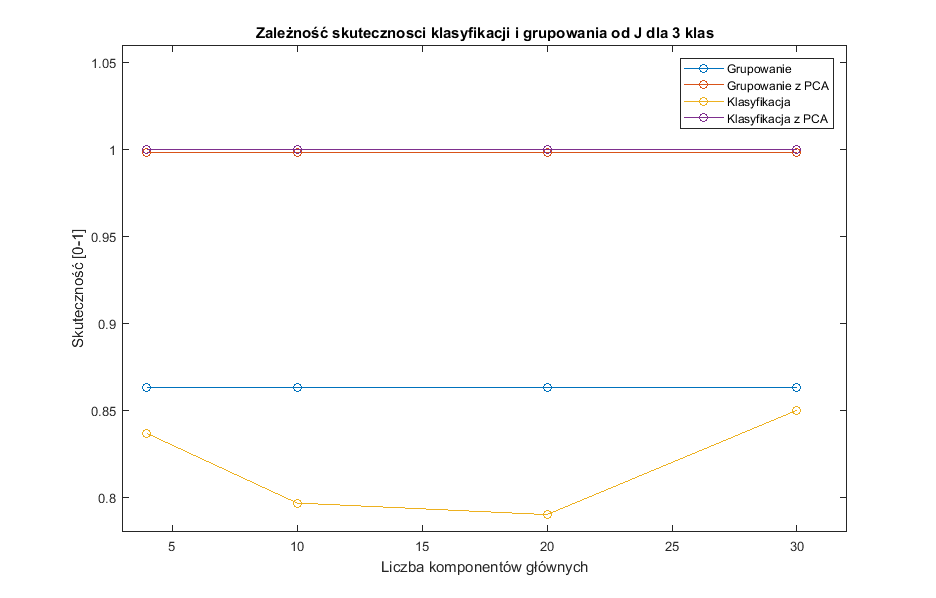
\includegraphics[scale = 0.7]{img/acc_from_J_3classes.png}
	\caption{Skuteczność grupowania i klasyfikacji dla 3 klas}  
	\label{rys:acc_from_J_3classes} 
\end{figure}

\begin{figure}[H]
	\centering
	\hspace*{-0.8in}
	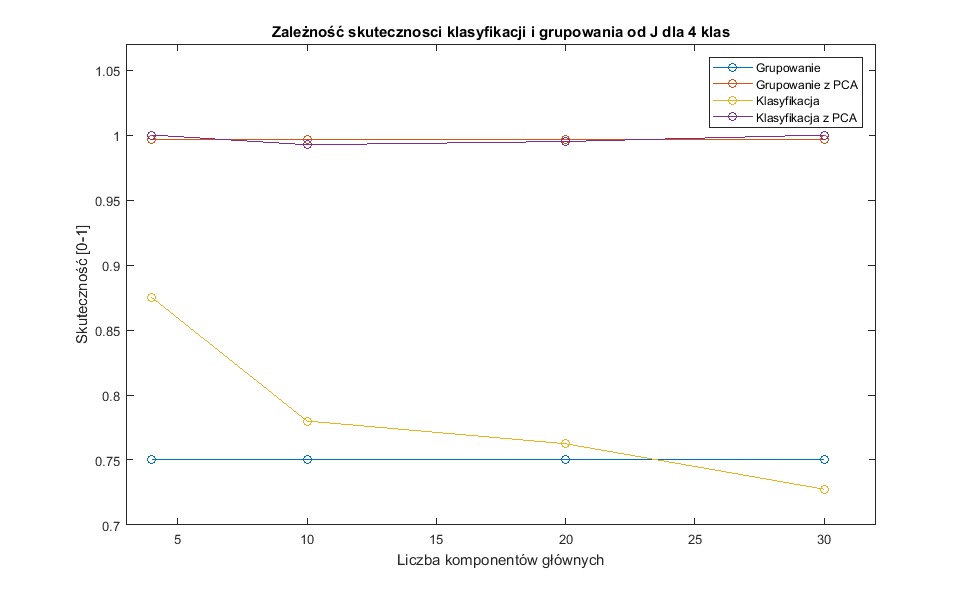
\includegraphics[scale = 0.7]{img/acc_from_J_4classes.png}
	\caption{Skuteczność grupowania i klasyfikacji dla 4 klas}  
	\label{rys:acc_from_J_42classes} 
\end{figure}

\begin{figure}[H]
	\centering
	\hspace*{-0.8in}
	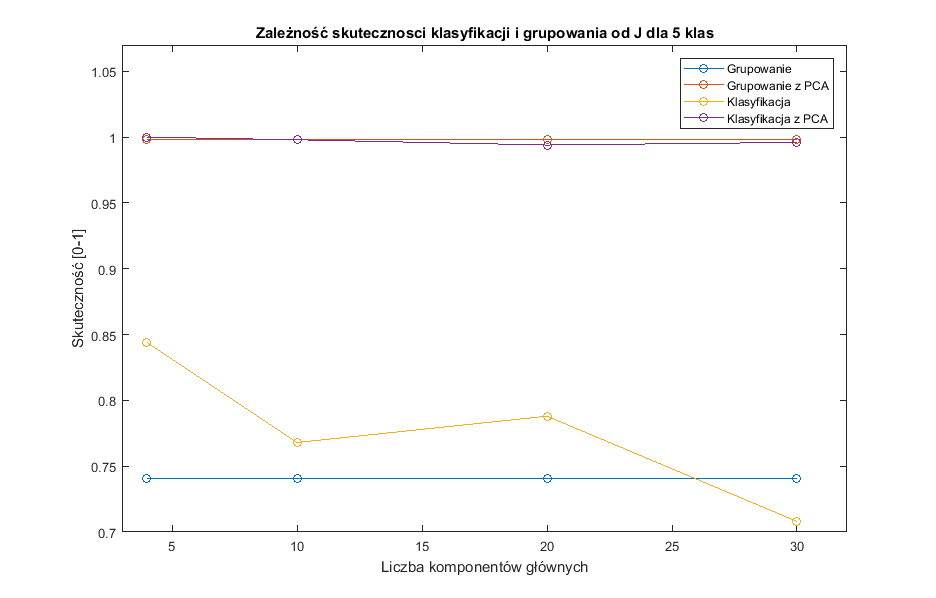
\includegraphics[scale = 0.7]{img/acc_from_J_5classes.png}
	\caption{Skuteczność grupowania i klasyfikacji dla 5 klas}  
	\label{rys:acc_from_J_5classes} 
\end{figure}